

\lecture{Memória}{mem}
\lecturetitle{\insertlecture}{\course}

\frame{\maketitle}

\part{Main Part}
\frame{\frametitle{Trilha}\tableofcontents[part=1]}

\section{Introdução}

\framevonneumannarch{}

% \begin{frame}
% \frametitle{Alocação de memória}

% \begin{columns}

% \begin{column}{0.5\textwidth}
% \input{img/memory-allocation}
% \end{column}

% \begin{column}{0.5\textwidth}
% \small
% \begin{tabbing}
% stru\=ct S \{\\
% 	\>float c;\\
% 	\>float d;\\
% \}\\
% main() \{\\
% 	\>{\color{blue}static int a};\\
% 	\>{\color{green!30!black} int b};\\
% 	\>struct S *s;\\

% 	\>{\color{red}s = (struct S*)(malloc(sizeof(struct S)))};\\
% \}\\
% \end{tabbing}

% \end{column}
% \end{columns}

% \end{frame}



\lecture{Hierarquia das memórias e conexões CPU-memória}{hierarchy}

\lecturetitle{\insertlecture}{\course}
\frame{\maketitle}

\section{\insertlecture}


\begin{frame}
  \frametitle{Tecnologias de memória}

  \def\headcolor{blue!80!black}

  \begin{tabular}[h]{c|c|c} \hline 
    {\color{\headcolor}{Tecnologia}} &
    {\color{\headcolor}{Tempo de acesso}} & {\color{\headcolor}{US\$
        por GB (2012)}}\\ \hline
    SRAM & 0,5--2,5 ns& \$500--\$1.000\\
    DRAM & 50-70 ns& \$10--\$20\\
    Flash & 5.000-50.000 ns& \$0,75--\$1\\
    Disco magnético & 5.000.000 -- 20.000.000 ns & \$0,05-\$0,10\\ \hline
  \end{tabular}
\noindent{\tiny Fonte: \emph{Computer Organization and Design}, 5th edition. Patterson \& Hennessy.
Morgan Kaufmann publishers.}

\bigskip\small
\noindent RAM--\emph{Random Access Memory} $\equiv$ Memória de Acesso Aleatório\\
\noindent SRAM--\emph{Static} RAM\\
\noindent DRAM--\emph{Dynamic} RAM\\

\end{frame}

\begin{frame}
  \frametitle{Hierarquia das memórias}

\begin{tikzpicture}[scale=0.6,head/.style={color=purple,anchor=center},
  labelsty/.style={anchor=center},mem/.style={fill=green!50!black},
  memtext/.style={color=white,midway},
  proc/.style={fill=gray!50!black}]
 
  \draw node[labelsty] at (13,7.1) {\bf tecnologia};
  \draw node[labelsty] at (9.25,7.1) {\bf custo};
  \draw node[labelsty] at (6,7.05) {\bf capacidade};
  \draw[proc] (2,6.25) rectangle (4,7.75) node[memtext]{\tiny{Processador}};
  \draw node[labelsty] at (-1,7.1) {\bf velocidade};

  \draw node[labelsty] at (13,5) {SRAM}; 
  \draw node[labelsty] at (9.25,5.1) {\Large{maior}};
  \draw node[labelsty] at (6.1,5) {\small{menor}};
  \draw[mem] (2.25,4.5) rectangle (3.75,5.25) node[memtext]{\tiny{Memória}};
  \draw node[labelsty] at (-1,5) {mais rápida};

  \draw node[labelsty] at (13,2) {DRAM};
  \draw[mem] (2,1.25) rectangle (4,2.75) node[memtext]{\scriptsize{Memória}};

  \draw node[labelsty] at (13,-2.1) {\small disco magnético/flash};
 \draw node[labelsty] at (9.25,-2.1) {\small{menor}};
  \draw node[labelsty] at (6.5,-2) {\Large{maior}};
  \draw[mem] (1.5,-3) rectangle (5,0) node[memtext]{Memória};
  \draw node[labelsty] at (-1,-2.1) {mais lenta};

\end{tikzpicture}

\end{frame}


\begin{frame}{Níveis da hierarquia de memória\footnote{\tiny Fonte: Computer
    Architecture. Hennessy \&
    Patterson. \href{http://www.isbnsearch.org/isbn/9780123704900}{ISBN
    13: 9780123704900}}}
  \begin{tikzpicture}[]
    \node[radius=3pt,circle,draw=blue] (cpu) {\color{blue}{CPU}};
    \node[draw,fill=lightgray] (reg) [below of=cpu,yshift=.5cm] {\tiny registradores};
    \node[minimum width=1.5cm,draw,fill=lightgray] (cache) [right=of
    cpu] {\scriptsize Cache};
    \draw (cpu) -- (cache);
    \node[minimum height=2cm,minimum width=2cm,draw,fill=lightgray]
    (mem) [right=of cache] {Memória};
    \draw (cache) -- (mem);
    \node[align=center,text width=2cm, ellipse,draw,fill=lightgray] (io) [right=of mem] {Dispositivos de E/S};
    \draw (mem) -- (io);

    \node[text width=2cm, align=center] [below of=cpu,yshift=-1cm]
    {\scriptsize 500 bytes 250 ps};
    \node[text width=1cm, align=center] [below of=cache,yshift=-1cm]
    {\scriptsize 64 KB 1 ns};
    \node[text width=1cm, align=center] [below of=mem,yshift=-1cm]
    {\scriptsize 1 GB 100 ns};
    \node[text width=1cm, align=center] [below of=io,yshift=-1cm]
    {\scriptsize 1 TB 10 ms};
  \end{tikzpicture}
\end{frame}


\begin{frame}{Terminologia\footnote{\tiny Fonte: \tocciref}}
  \framesubtitle{Endereços de memória e dados}
  \newcounter{wordno}\setcounter{wordno}{0}

\begin{columns}
\begin{column}{0.5\textwidth}
\scriptsize
\begin{block}{Terminologia}
  \begin{description}
  \item[Célula de memória:] dispositivo ou circuito elétrico utilizado
    para armazenar um único bit;
  \item[Palavra:] grupo de bits (células) que representa instruções ou dados;
  \item[Byte:] termo para grupo de 8 bits;
  \item[Capacidade:] especificação da quantidade de bits armazenada em
    um dispositivo de memória;
  \item[Endereço:] número que identifica a posição de uma palavra na memória.
  \end{description}
  
\end{block}
\end{column}

\begin{column}{0.5\textwidth}
  \begin{center}
  \begin{tikzpicture}
    \node[fill=lightgray] at (0,.5) {\small Endereço};
    \node[] (memcel) at (1.75,1) {\tiny células de
      memória (bits)};
    \draw[->,>=latex] (memcel) -- (1.45,0.25);
    \draw[->,>=latex] (memcel) -- (1.85,0.25);
    \foreach \x in {0,...,7} {
      \node[minimum height=.5cm,minimum width=0.21,fill=lightgray,draw] at (1+.215*\x,0) {};
    }
    \foreach \a in {0,1} {
      \addtocounter{wordno}{\a};
      \foreach \b in {0,1} {
         \addtocounter{wordno}{\b};
        \foreach \c in {0,1} {
          \addtocounter{wordno}{\c};
           \node[fill=lightgray,minimum width=2] at (0,-\a*.5-\b*1-\c*2) {\c\b\a};
           \node[draw] at (1.75,-2*\a-\b-.5*\c) {Palavra
             \arabic{wordno}};
           \draw[->,>=latex,color=gray] (.5,-0.5*\a-\b-2*\c) -- (.75,-0.5*\a-\b-2*\c);
         }
       }
     }
  \end{tikzpicture}
\end{center}
\end{column}

\end{columns}
\end{frame}


\begin{frame}{Conexões CPU-memória\footnote{\tiny Fonte: \tocciref}}

\begin{center}
  \begin{tikzpicture}[memsty/.style={minimum width=1.75cm,minimum
      height=1.25cm,draw}, bussty/.style={color=black!50!green}]
    \node[minimum width=1cm,minimum height=3cm,draw] (cpu) {CPU};
    \draw[->,>=latex] (cpu.north east) -> +(1,0) node[] (a0) {};
    % barramento de endereco
    \node [above of=a0,xshift=.5cm,yshift=-.75cm,bussty] {\tiny barramento de endereço};
    \draw[] (a0.center) -- +(4,0) node (a1) {};
    \draw[dashed] (a1) -- +(2,0);
    \draw[->,>=latex] (a0.west)+(1,0) -- +(1,-.5) node (amem0) {};
    \draw[->,>=latex] (a0.west)+(3,0) -- +(3,-.5) node[anchor=south] (amem1) {};
    \node[memsty] [below of=amem0,yshift=.39cm] {\color{blue}{memória}};
    \node[memsty] [below of=amem1,yshift=.25cm]
    {\color{blue}{memória}};
    \draw[->,>=latex] (cpu.south east)+(0,.5) -> +(1,0.5) node[] (a2) {};
    \draw[<-,>=latex] (cpu.south east)+(0,.5) -> +(1,0.5) node[] (a3)
    {};
    
    % barramento de dados
    \draw[] (a3.center) -- +(4,0) node (a4) {};
    \draw[dashed] (a4) -- +(2,0);
    \draw[->,>=latex] (cpu.south east)+(0,.1) -> +(1,0.1) node[] (a5)
    {};
    \draw[->,>=latex] (a3.west)+(1,0) -- +(1,.79) node (amem0) {};
    \draw[->,>=latex] (a3.west)+(3,0) -- +(3,.79) node[anchor=south] (amem1) {};
    \draw[<-,>=latex] (a3.west)+(1.5,0) -- +(1.5,.79) node (amem0) {};
    \draw[<-,>=latex] (a3.west)+(3.5,0) -- +(3.5,.79) node[anchor=south] (amem1) {};
    \node [text width=1cm,below of=a4,xshift=-4.45cm,yshift=1.45cm, bussty] {\tiny barramento de dados};

    % barramento de controle
    \draw[] (a5.center) -- +(4,0) node (a6) {};
    \draw[dashed] (a6) -- +(2,0);
    \draw[->,>=latex] (a5.west)+(.7,0) node (joint0) {} -- +(.7,1.19)
    node (amem0) {};
    \fill  (joint0) circle [radius=0.05];
    \draw[->,>=latex] (a5.west)+(2.7,0) node (joint1) {} -- +(2.7,1.19)
    node[anchor=south] (amem1) {};
    \fill  (joint1) circle [radius=0.05];
    \node [below of=a6,xshift=-3.5cm,yshift=.75cm, bussty] {\tiny barramento de controle};
  \end{tikzpicture}
\end{center}

\end{frame}


\begin{frame}{Operações: Escrita ({\tt $\overline{WR}|R\overline{W}$})}
  
  Código MIPS: \hfil{\tt sw \$s0, 0(\$s1)}\hfill\\\bigskip

  \begin{enumerate}[<+-| alert@+>]\setbeamercovered{transparent}
  \item A CPU fornece o {\bf endereço} em que o dado será armazenado
    utilizando as linhas do barramento de endereço;
  \item A CPU coloca os {\bf dados} a serem armazenados nas linhas do
    barramento de dados;
  \item A CPU ativa as linhas do sinal de {\bf controle} apropriado ({
      $\overline{WR}$ ou $R\overline{W}$});
  \item Os dados no barramento são {\bf transferidos} para a posição de
    memória selecionada.
  \end{enumerate}
  
\end{frame}

\begin{frame}{Operações: Leitura}
  Código MIPS: \hfil{\tt lw \$t0, 0(\$s1)}\hfill\\\bigskip

  \begin{enumerate}[<+-| alert@+>]\setbeamercovered{transparent}
  \item A CPU fornece às linhas de {\bf endereço}, o valor binário a partir
    do qual os dados devem ser recuperados;
  \item A CPU ativa as linhas de controle adequadas para a operação de
    leitura na memória ({$\overline{RD}$});
  \item Os circuitos de memória {\bf transferem} os dados da posição
    requisitada no barramento de dados, que são enviados para a CPU.
  \end{enumerate}
\end{frame}

\begin{frame}{Funções dos barramentos}

  \begin{description}[<+-| alert@+>]\setbeamercovered{transparent}
  \item[Barramento de endereço:] é {\bf unidirecional} e transporta os
    sinais contendo endereços da CPU para os circuitos de memória;
  \item[Barramento de dados:] é {\bf bidirecional} transportando os
    dados da CPU para os circuitos de memória e vice-versa;
  \item[Barramento de controle:] Transporta os sinais de controle
    ({$\overline{RD}$, $\overline{WR}$}) da
    CPU para os circuitos de memória.
  \end{description}
  
\end{frame}

\lecture{Memórias RAM e ROM}{RAMROM}
\frame{\maketitle}

\section{\insertlecture}

\begin{frame}{Memória de acesso aleatório -- RAM}{\em Random Access
    Memory}
  \begin{itemize}
  \item Armazenamento temporário de programas em execução e dados;
  \item Tipos
    \begin{itemize}
    \item<1-> Dinâmica (DRAM -- {\em Dynamic} RAM): baixo custo, grande
      capacidade de armazenamento, pouco consumo de energia, porém,
      precisam ser alimentadas constantemente por um sinal chamado
      {\em refresh}, daí seu nome dinâmica. São usados capacitores
      para a sua construção.
      \note[item]{Como os capacitores tem perda de carga ao longo do
        tempo há a necessidade de refresh.}
    \item<2> Estática (SRAM -- {\em Static} RAM): tempo de acesso
      pequeno, alto custo e não precisam de pulso de {\em refresh}. Em vez
      de capacitores, são usados circuitos chamados {\em flip-flops}
      que dispensam ciclos de {\em refresh}, porém, consomem muita
      energia.  
      \note[item]<2>{Apesar de comumente chamarmos a DRAM de
        RAM a SRAM também é RAM, o mais correto seria chamarmos a DRAM
        de memória principal.}
    \end{itemize}
  \end{itemize}  
  
\end{frame}

\begin{frame}{Célula RAM Dinâmica}{{\em Dynamic Ram}}
\begin{figure}
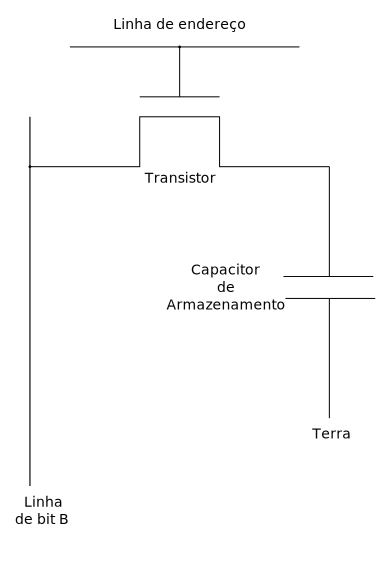
\includegraphics[scale=0.5]{img/mem-dram_cell.png}
\end{figure}
\end{frame}

\begin{frame}{Arranjo típico da célula de memória}
  \def\R{0.2}
\centering
\begin{tikzpicture}[scale=0.8]
  \foreach \x in {0,1,...,7} {
    \foreach \y in {0,1,...,7} {
      \node[circle,draw,radius=\R] (c\x\y) at (\x,\y) {};
      \draw (\x-\R*4,\y) -- (\x-\R,\y);
      \draw (\x,\y+\R*4) -- (\x,\y+\R);
    }
  }
  \foreach \x in {0,2,4,6} {
    \foreach \y in {5,7} {
      \node[circle,draw,radius=\R,fill=red] (c\x\y) at (\x,\y) {};
    }
  }
  \draw (-\R*4,-\R*4) -- (-\R*4,7+\R*2);
  \node at (\R*16, 7+\R*6) {\scriptsize endereço da coluna};
  \draw[->,>=latex]  (-\R*6, -\R*4) -- (-\R*6,-\R*2) node[left,
  text width=2cm]  {\tiny controle de estado do capacitor};
  \draw (-\R*2,7+\R*4)  -- (7+\R*4,7+\R*4) ;
  \draw[->,>=latex]  (-\R*16, 7+\R*4) -- (-\R*4,7+\R*4) node[above left]
  {\scriptsize carga};
  \node[rotate=90] at (-\R*6,\R*16) {\scriptsize endereço da linha};
\end{tikzpicture}
\end{frame}

\begin{frame}{DRAM}
  \begin{itemize}[<+-| alert@+>]\setbeamercovered{transparent}
  \item A célula de memória representa um único bit de dado.
  \item As células são impressas em uma pastilha de silício.
  \item Vetor de colunas.
  \item Vetor de linhas.
  \item A intersecção entre a linha e a coluna é o endereço 
    da célula de memória.
  \item Mantem a integridade dos dados enviando um pulso  
    periódico para as células de memória.
  \end{itemize}  
\end{frame}

\begin{frame}{DRAM síncrona}{SDRAM -- {\em Synchronous} DRAM}
  \begin{itemize}
  \item Utiliza o clock do barramento local para comandar os seus
    circuitos internos, sem necessidade de espera de sincronia com a
    placa-mãe.
  \item Como determinar a frequência?
    $\Rightarrow 15 ns =  {1000\over{15}} MHz = 66 MHz$
  \end{itemize}

\pause\bigskip\small
\noindent DDR--\emph{Double Data Rate} $\equiv$ Taxa Dupla de (transferência) Dados\\\bigskip

DDR4-3200 DRAM pode realizar 3.200 milhões de transferências por segundo, 
o que significa uma taxa de 1.600MHz.

\end{frame}


\section{Memória ROM}

\begin{frame}{Mem\'{o}ria somente-leitura}{Read-Only Memory -- ROM}

A memória \alert{ROM} contém um padrão permanente de dados
que não pode ser mudado, ou seja, \alert{não é volátil} 
e normalmente é usada nas seguintes aplicações:

\begin{itemize}
\item Microprogramação;
\item Biblioteca de funções de uso frequente;
\item Programas do sistema;
\item Tabelas de função.
\end{itemize}

\end{frame}

\begin{frame}{ROM Programável}{Programmable ROM -- PROM}
\footnotesize
\begin{description}
\item[EPROM -- \textit{Erasable PROM}:] \alert{EPROM apagável} é 
lida e escrita eletricamente, porém, antes da operação de escrita
todas as células precisam ser apagadas para retornar ao estado 
inicial. A operaç\~ao de apagamento \'{e} realizada utilizando
luz ultra-violeta.
\pause
\item[EEPROM -- \textit{Eletrically Erasable PROM}:] 
\alert{PROM apagada eletricamente} \'e utilizada principalmente
para leitura que pode ser escrita sem apagamento de todo o 
conte\'{u}do, apenas o byte ou bytes endereçados s\~ ao
atualizados. A EEPROM é mais cara que EPROM e também menos
densa, adminitindo menos bits por chip.
\pause
\item[Memória \textit{flash}:] intermedi\'{a}ria entre a
EPROM e EEPROM tanto no custo quanto na funcionalidade. 
Assim como a EEPROM, a mem'oria \textit{flash} usa uma tecnologia
el\'{e}trica de apagamento. A mem\'{o}ria pode ser apagada
completamente em alguns segundos. Al\'em disso, \'{e} 
poss\'{i}vel apagar blocos de mem\'{o}ria ao inv\'es da 
mem\'oria inteira. Por\'em, a mem\'oria \textit{flash} n\~ao
oferece apagamento em n\'ivel de byte. Assim como a EPROM,
utiliza um transistor por bit tendo alta densidade quando
comparada com a EEPROM. (Ex: pendrive)
\end{description}
\end{frame}


\begin{frame}{Tecnologias utilizadas}

As mudanças nas tecnologias utilizadas buscar reduzir o tempo de
resposta da memória, para reduzir o tempo de espera do processador e
níveis intermediários de memória {\it cache\/}.

\begin{itemize}
\item
  \href{http://www.hardware.com.br/livros/hardware/tecnologias-utilizadas.html}
  {Recursos adicionais:\\{\tt hardware.com.br/livros/hardware$\Rightarrow$} Livro online
    ``Hardware, o Guia Definitivo'', \\capítulo de ``Memórias: Tecnologias utilizadas''}
\end{itemize}

\end{frame}

%%%%%%%%%%%%%%%%%%%%%%%%%%%%%%%%%%%% CACHE %%%%%%%%%%%%%%%%%%

\lecture{Memória Cache}{cache}
\title{\insertlecture}
\frame{\maketitle}

\section{\insertlecture}

% layout simples do caminho cache -> barramento -> memoria
\def\cachebusmem{
\begin{tikzpicture}
		\tikzset{dev/.style={draw},com/.style={>=latex}}
		\node[dev] (p) {processador};
		\node[dev] (c) [right of=p,xshift=15mm] {cache};
		\node[dev,minimum height=3cm,minimum width=.25cm,fill=black] (b) [right of=c,xshift=12.5mm] {};
		\node[] [above of=b,yshift=10mm] {barramento};
		\node[dev,minimum height=1.75cm] (m) [right of=b,xshift=15mm,text width=1.5cm] {memória principal};		
		

		\draw[<->,com] (p) -- (c);
		\draw[<->,com] (c) -- (b);
		\draw[<->,com] (b) -- (m);
\end{tikzpicture}
}	


\frame{
\frametitle{Mem\'oria: princ\'ipios f\'isicos}
Revis\~ao:\\
\begin{itemize}
	\item Hierarquia de memória;
	\item Mem\'oria RAM: est\'atica, din\^ amica;
	\item Mem\'oria ROM: PROM, EPROM, EEPROM;
	\item Mem\'oria flash.
\end{itemize}
}

\section{Mem\'oria: fundamentos l\'ogicos}
\frame{
\frametitle{Mem\'oria: fundamentos l\'ogicos}
	O layout de mem\'oria visa equilibrar a
	relação entre a hierarquia de memória,
	acesso e consistência dos dados e performance.
	Juntamente com o layout são projetados algoritmos
	de substituição de blocos de memória para conseguir
	melhorias na performance.

\bigskip
	Estes algoritmos normalmente levam em conta 
	a frequência de acesso dos dados para a definição
	de políticas de substituição dos blocos de memória.
	Princ\'ipio da localidade:
	\begin{itemize}
		\item Temporal
		\item Espacial
	\end{itemize}

}


\def\thetitle{Introdução}
\section{\thetitle}

\begin{frame}{Cache única}{cache e memória principal}
  \begin{tikzpicture}
    \tikzset{proc/.style={draw,fill=gray!60!white},cache/.style={proc,minimum
        width=2.5cm,minimum height=1.25cm,fill=red!50!black,text=white},ram/.style={cache, minimum
        width=4cm, minimum height=2cm,fill=green!25!black,text=white}}
    \node[proc] (p) {\bf processador};
    \node[cache] (c) [right of=p,xshift=25mm] {\bf cache};
    \node[ram] (r) [right of=c,xshift=35mm] {\bf memória principal (RAM)};

    \draw[<->,>=latex] (p) -- node[below] (f) {\footnotesize rápida} (c) ;
    \draw[<->,>=latex] (c) -- node[below] (l) {\footnotesize lenta} (r) ;

    \node[draw,double] [above of=f,xshift=-2.5mm] {\footnotesize
      palavra};
    \node[draw,double,minimum height=1cm] [above of=l,xshift=-2.5mm,yshift=5mm] {\footnotesize bloco};

  \end{tikzpicture}
  
\end{frame}

\begin{frame}{Cache em três níveis}{cache e memória principal}
  \scriptsize
  \begin{tikzpicture}
    \tikzset{proc/.style={draw,fill=gray!60!white},cache/.style={proc,minimum
        width=1.25cm,minimum
        height=1.25cm,fill=red!50!black,text=white,text
        width=1.25cm},ram/.style={cache, minimum
        height=6cm,fill=green!25!black,text=white}} \node[proc] (p)
    {\bf processador}; \node[cache] (c1) [right
    of=p,xshift=12.5mm] {\bf cache de nível 1 (L1)};
    \node[cache,minimum height=2cm] (c2) [right
    of=c1,xshift=15mm] {\bf cache de nível 2 (L2)};
    \node[cache,minimum height=3cm] (c3) [right of=c2,xshift=15mm]
    {\bf cache de nível 3 (L3)}; \node[ram] (r)
    [right of=c3,xshift=15mm] {\bf memória principal (RAM)};

    \draw[<->,>=latex] (p) --
    node[below,xshift=-2.5mm,yshift=-2.5mm,text width=1cm]
    {\scriptsize mais rápida} (c1) ;
    \draw[<->,>=latex] (c1) -- node[below] {\scriptsize rápida}
    (c2) ;
    \draw[<->,>=latex] (c2) -- node[below,text width=1cm] {\scriptsize menos rápida} (c3) ;
    \draw[<->,>=latex] (c3) -- node[below] {\footnotesize lenta} (r) ;

  \end{tikzpicture}
  
\end{frame}


\def\thetitle{Mapeamento DRAM $\Rightarrow$ cache}

\section{\thetitle}

\frame{\frametitle{Requisiç\~ao de dados pelo processador}
	\cachebusmem}

\subsection{Mapeamento entre memória cache e principal}
% key of each block in bits to be mapped
\pgfkeyssetvalue{/mem/0}{000}
\pgfkeyssetvalue{/mem/1}{001}
\pgfkeyssetvalue{/mem/2}{010}
\pgfkeyssetvalue{/mem/3}{011}
\pgfkeyssetvalue{/mem/4}{100}
\pgfkeyssetvalue{/mem/5}{101}
\pgfkeyssetvalue{/mem/6}{110}
\pgfkeyssetvalue{/mem/7}{111}
% memory tags
\pgfkeyssetvalue{/tag/0}{00}
\pgfkeyssetvalue{/tag/2}{01}
\pgfkeyssetvalue{/tag/4}{10}
\pgfkeyssetvalue{/tag/6}{11}
\pgfkeyssetvalue{/tag/xx}{}%tag associated with index


\def\height{2} % height of each block of memory
\def\width{0.25} % width of each block of memory
\def\drawmem#1#2#3#4{ % #1 - x position, #2 - y position, #3 - is cache?
                    % 1 is yes, #4 - tag, xx if its cache
  \foreach \i in {0,1,...,7} {
    \def\memnode{node[] at
      (#1+\i*\width+\width/2,#2-\width/2) {\tiny{\pgfkeysvalueof{/tag/#4}\underline{\pgfkeysvalueof{/mem/\i}}}}}
    \def\color{white}
    \ifnum\i=1
    \def\color{red}
    \else
    \ifnum\i=5
    \def\color{blue!60!black}
    \else
    \def\memnode{node{}}
    \fi
    \fi
    
    \ifnum#3=1%
    \def\memnode{node[rotate=90] at (#1+\i*\width+\width/2,#2+\height+\width) {\tiny{\pgfkeysvalueof{/mem/\i}}}}
    \fi

    \draw[fill=\color] (#1+\i*\width,#2) rectangle
    (#1+\i*\width+\width,#2+\height) \memnode;
    
    % label the center of each rectangle
    \node[] (\pgfkeysvalueof{/tag/#4}\pgfkeysvalueof{/mem/\i}) at
    (#1+\i*\width+\width/2,#2+\height/2) {};
  } % foreach i 
} % \def ...

\begin{frame}
  \frametitle{Mapeamento direto}
  
  \begin{tikzpicture}[scale=1.1,line width=0.5pt]
    
    \node[] at (4,3+\height+3*\width) {cache};

    \drawmem{3}{3}{1}{xx}
    \foreach \j in {0,2,4,6} {
      \drawmem{\j}{0}{0}{\j}
      
      \foreach \z in {1,5} {
        \fill (\pgfkeysvalueof{/tag/\j}\pgfkeysvalueof{/mem/\z})
        circle (1pt);
        \draw[->] (\pgfkeysvalueof{/tag/\j}\pgfkeysvalueof{/mem/\z}) to
        (\pgfkeysvalueof{/tag/xx}\pgfkeysvalueof{/mem/\z});
      } % foreach z 
    } % foreach j ...
    
    \node[] at (16*\width,-0.75) {memória};
    
  \end{tikzpicture}

\end{frame}

\def\memory#1{Memory(#1)}
\def\blue#1{\color{blue!60!black}{#1}}

\begin{frame}
  \frametitle{Exemplo}
  
    Processador requisita o endereço $\rightarrow$
    \only<1>{\tt 10\alert{\pgfkeysvalueof{/mem/6}}}
    \only<3>{\tt 11\alert{\pgfkeysvalueof{/mem/2}}}
    \only<5>{\tt 11\alert{\pgfkeysvalueof{/mem/0}}}
    \only<7>{\tt 00\alert{\pgfkeysvalueof{/mem/3}}}
    \only<10-11>{\tt 10\alert{\pgfkeysvalueof{/mem/2}}}
    \bigskip

  \begin{tabular}[h]{|c|c|c|c|}\hline
    índice & válido? & etiqueta~\footnote{tradução livre de \em tag} & dados \\ \hline
    %%%% 0
    \alert<5>{\pgfkeysvalueof{/mem/0}} 
    & 
    \only<1-4>{\color{red}{F}} \only<5->{V} 
    & 
    \only<6>{\blue{\pgfkeysvalueof{/tag/6}}}
    \only<7->{\pgfkeysvalueof{/tag/6}}
    & 
    \only<6>{\blue{\memory{\pgfkeysvalueof{/tag/6}\pgfkeysvalueof{/mem/0}}}}
    \only<7->{\memory{\pgfkeysvalueof{/tag/6}\pgfkeysvalueof{/mem/0}}}
    \\ \hline
    %%%% 1
   \pgfkeysvalueof{/mem/1} & \color{red}{F} & & \\ \hline

   %%%% 2
   \alert<3,11>{\pgfkeysvalueof{/mem/2}} 
   & 
   \only<1-3>{\color{red}{F}} \only<4->{V}
   & 
   \only<4>{\blue{\pgfkeysvalueof{/tag/6}}}
   \only<5-10>{\pgfkeysvalueof{/tag/6}}
   \only<11>{\color{gray}\pgfkeysvalueof{/tag/6}}
   \only<12>{\blue{\pgfkeysvalueof{/tag/4}}}
   \only<13->{\pgfkeysvalueof{/tag/4}}
   &
   \only<4>{\blue{\memory{\pgfkeysvalueof{/tag/6}\pgfkeysvalueof{/mem/2}}}}
   \only<5-10>{\memory{\pgfkeysvalueof{/tag/6}\pgfkeysvalueof{/mem/2}}} 
   \only<11>{\color{gray}\memory{\pgfkeysvalueof{/tag/6}\pgfkeysvalueof{/mem/2}}} 
   \only<12>{\blue{\memory{\pgfkeysvalueof{/tag/4}\pgfkeysvalueof{/mem/2}}}}
   \only<13->{\memory{\pgfkeysvalueof{/tag/4}\pgfkeysvalueof{/mem/2}}} 
   \\ \hline

   %%%% 3
   \alert<7>{\pgfkeysvalueof{/mem/3}}
   & 
   \only<1-5>{\color{red}F} \only<6->{V} 
   & 
   \only<8>{\blue{\pgfkeysvalueof{/tag/0}}}
   \only<9->{\pgfkeysvalueof{/tag/0}}
   & 
   \only<8>{\blue{\memory{\pgfkeysvalueof{/tag/0}\pgfkeysvalueof{/mem/3}}}}
   \only<9->{\memory{\pgfkeysvalueof{/tag/0}\pgfkeysvalueof{/mem/3}}}
   \\ \hline

   %%%% 4
   \pgfkeysvalueof{/mem/4}    & \color{red}{F} & & \\ \hline

   %%%% 5
   \pgfkeysvalueof{/mem/5}    & \color{red}{F} & & \\ \hline

   \alert<1>{\pgfkeysvalueof{/mem/6}} & \only<1>{\color{red}{F}} \only<2->{V}
   & 
   \only<2>{\blue{\pgfkeysvalueof{/tag/4}}}
   \only<3->{\pgfkeysvalueof{/tag/4}}
   &
   \only<2>{\blue{\memory{\pgfkeysvalueof{/tag/4}\pgfkeysvalueof{/mem/6}}}}
   \only<3->{\memory{\pgfkeysvalueof{/tag/4}\pgfkeysvalueof{/mem/6}}} \\ \hline

   %%%% 6
   \pgfkeysvalueof{/mem/7}    & \color{red}{F} & & \\ \hline
 \end{tabular}

\end{frame}

\begin{frame}{Busca na memória cache}{}
 
{\color{blue} \em cache hit -- } presença do dado requisitado na cache.  
\alert{\em cache miss -- } ausência do dado requisitado na cache.  \\
\small Estratégia utilizada da ausência do dado na cache:
\begin{enumerate}
\item Enviar o valor original do contador (atual {\tt PC}$-4$) para a memória.
\item Instruir a memória principal a realizar esta leitura e esperar pelo 
término do acesso.
\item Escrever a entrada na cache, colocando o dado da memória na porção
da entrada, escrevendo os bits mais significativos do endereço (da ULA) no 
campo de marcação (\textit{tag}), e ligando (V) o bit de válido.
\item Reiniciar a instrução de execução do primeiro passo, que irá recuperar
o dado que agora está na cache.
\end{enumerate}
 \end{frame}


\def\w{0.4cm}
\def\filltext{}
\def\tag{}
\def\memlocation#1{% 0=direct mapped, 1=set associative, 2=fully associative
\tikzset{data/.style={draw,minimum height=2cm,minimum width=0.4cm},
	tag/.style={data,minimum height=1cm}}
	
	\def\mark{}
	\ifnum#1=0      
      	\def\mark{4}
	\fi    
    \ifnum#1=1  	
     	\def\mark{1}
	\fi	
	\ifnum#1=2     	
     	\def\mark{6}
     \fi
      
      \def\drawmark{\draw[<-,>=latex] (tag\z) -- (search\z);}
      \foreach \z in {0,1,2,3,4,5,6,7} {
		\ifnum\z=\mark
			\def\filltext{fill}
			 \def\tag{\footnotesize 0}
		\fi      
      				
		\node[data,\filltext] (d\z) at (\w*\z,0) {};
		\node (bl\z) [above of=d\z,yshift=2.5mm] {\small \z};
		\node[tag] (tag\z) at  (\w*\z,-2) {\tag};			
		\node (search\z) [below of=tag\z,yshift=-1mm] {};		

		% direct mapped
		\ifnum#1=0
			\ifnum\z=\mark
				\drawmark
			\fi
		\fi				
		% set associative
		\ifnum#1=1
			\ifnum\z=0
				\drawmark
			\fi
			\ifnum\z=1
				\drawmark
			\fi
		\fi			
		% fully associative
		\ifnum#1=2
			\drawmark
		\fi	   
	   }
	\fill[blue,opacity=0.5] (d4);	
	\node [left of=bl0] {Bloco};
	\node [left of=d0] {Dado};
	\node (tl) [left of=tag0] {Tag};
	\node [below of=tl] {Busca};	
} 


 \begin{frame}
  \frametitle{Estratégias mais flexíveis}
	\only<2->{Objetivo: reduzir a ausência de dados na memória cache. }
 
  \begin{itemize}
  \item<1,2> {\only<2>{\color{gray}}Mapeamento direto}
  \item<2,3> \textbf{Mapeamento em conjunto} -- o bloco pode ser colocado em um conjunto
  de locais na memória cache. 
  \item<2,4> \textbf{Sem mapeamento} -- o bloco pode ser colocado em qualquer local
  na memória cache.
  \end{itemize}

	\only<1>{
	\begin{tikzpicture}
	\memlocation{0}				
	\end{tikzpicture}
  }
  
  \only<3>{
	\begin{tikzpicture}
	\memlocation{1}				
	\end{tikzpicture}
  }
  \only<4>{
    \begin{tikzpicture}
		\memlocation{2}					
	\end{tikzpicture}
  }
\end{frame}
	

\begin{frame}
  \frametitle{Gravação em memória cache}
	
  \begin{itemize}
  \item<1,2> \textbf{\em write-through}\only<2>{ -- sempre escrever o dado na memória principal 
  e cache.}
  \item<1,3> \textbf{\em write buffer} \only<3>{fila para armazenar o dado enquanto o
  dado está esperando para ser escrito na memória.}
  \item<1,4> \textbf{write-back} \only<4>{ -- sempre escreve o dado no bloco,
  se o dado for modificado, este é gravado na memória em um nível mais
  baixo da hierarquia. Este esquema pode melhorar a performance, porém,
  é mais complexo de ser implementado.}
  \end{itemize}

	\only<2>{
	\begin{center}
		\cachebusmem%
	\end{center}
	}
	\only<3>{
	\begin{center}
	\begin{tikzpicture}[dev/.style={draw},com/.style={>=latex}]
		\node[dev] (p) {processador};
		\node[dev] (c) [right of=p,xshift=15mm] {cache};
		\node[dev,minimum height=1cm] (bf) [below of=c,yshift=-5mm] {buffer};
		\node[dev,minimum height=3cm,minimum width=.25cm,fill=black] (b) [right of=bf,xshift=12.5mm] {};
		\node[] [above of=b,yshift=10mm] {bus};
		\node[dev,minimum height=1.75cm] (m) [right of=b,xshift=15mm,text width=1.5cm] {memória principal};		
		

		\draw[<->,com] (p) -- (c);
		\draw[<->,com] (c) -- (bf);
		\draw[<->,com] (bf) -- (b);
		\draw[<->,com] (b) -- (m);
	\end{tikzpicture}
	\end{center}
	}

\end{frame}


\framemipsprocfigure{}

%% \begin{frame}{Estudo de caso: Processador Intel® Core™
%%     i7-2600\footnote{\scriptsize Fonte: \url{http://ark.intel.com/Product.aspx?id=52213}}}
%% {Sandy Bridge}
%% \scriptsize

%% \only<1>{
%% \begin{columns}
%%   \begin{column}{.375\textwidth}
%%     \begin{tabular}{|l|l|}\hline
%%       N$^o$ de núcleos & 4 \\
%%       N$^o$ de {\em threads} & 8 \\
%%       Frequência do {\em clock} & 3.4 GHz \\
%%       Intel® Smart Cache & 8 MB\\\hline
%%     \end{tabular}
%%   \end{column}
  
%%   \begin{column}{.5\textwidth}
%%    \begin{tabular}{|l|l|}\hline
%%       Conjunto de instruções & 64 bits\\
%%       Litografia & 32 nm \\
%%       Máxima potência dissipada & 95 W \\\hline
%%     \end{tabular}
%%     \end{column}
%% \end{columns}
%% }
%% \only<2>{
%% \begin{itemize}
%% \item   Cache L1 de instruções de 32 kB e cache L1 de dados de 32 kB por núcleo (nenhuma mudança em relação à arquitetura Nehalem)
%% \item O cache de memória L2 foi renomeado para “cache intermediário” (MLC, Mid-Level Cache) com 256 kB por núcleo
%% \item O cache L3 agora é chamado “cache de último nível” (LLC, Last Level Cache) é compartilhado entre os núcleos do processador e o processador gráfico.
%%     \end{itemize}
%%     }
%% \begin{figure}
%% %    \includegraphics[scale=.275]{img/sandy-bridge-die-map-1024x512.png}
%%   \end{figure}

%% \end{frame}

%%%%%%%%%%%%%%%%%%%%%%%%%%%%%%%% VIRTUAL MEMORY

\lecture{Gerenciamento de memória}{mmu}

%\input{../../os/img/mm_mmu} % mmu draw

\title{\insertlecture}

\frame{\titlepage}

\begin{frame}{Unidade de gerenciamento de memória}
  \small
  A \alert{Unidade de Gerenciamento de Memória} converte endereços
  físicos da memória principal/primária (DRAM) para endereços lógicos
  utilizados pelo processador.

\bigskip

 % \mmudraw{0} % from os

\end{frame}

% \begin{frame}{Cache da MMU}

%     \mmudraw{1} % from os

% \end{frame}

\lecture{Memória Virtual}{vmem}
\section{\insertlecture}
\title{\insertlecture}

\frame{\maketitle}

\begin{frame}{\insertlecture}
\def\widthv{6}
\def\heightv{1}
\def\widthvalid{0.5}
\def\shift{7}% shift from virtual page
  
 {\footnotesize Implementa o mapeamento do \alert{espaço de endereçamento} dos
programas para \alert{endereços físicos} de memória.}
\bigskip

\begin{columns}
\begin{column}{.7\textwidth}
  \begin{tikzpicture}[scale=0.275]
    
    \node[draw,rectangle] (idv) at (-4.5,18) {\tiny{n$^o$ da página virtual}};
    \path[draw,->] (idv) -- (-4.5,7) -- (0,7);
   
    \newcounter{memcounter}\setcounter{memcounter}{0}
    \newcounter{hdcounter}\setcounter{hdcounter}{-2}
    \foreach \vv in {0,1,...,13} {
      \pgfsetfillopacity{0.5}
      \def\advancehd{\addtocounter{hdcounter}{-2}}
      \def\reccolor{white}
      \def\vbit{\tiny{1}}
      \def\hdmap{\def\reccolor{gray} \def\vbit{\tiny{0}};}
      \def\physmem{\draw[fill=gray] (\widthv+\shift,\arabic{hdcounter}+\widthv) rectangle
        (2*\widthv+\shift,\arabic{hdcounter}+\heightv+\widthv);
        \node[right] (mem\vv) at
        (\widthv+\shift,\arabic{hdcounter}+\widthv) {};}
      \ifnum\vv=1
      \hdmap \advancehd
      \else\ifnum\vv=4
      \hdmap \advancehd
      \else\ifnum\vv=7
      \hdmap \advancehd
      \else
      \def\physmem{\draw (\widthv+\shift,\arabic{memcounter}+\widthv) rectangle
        (2*\widthv+\shift,\arabic{memcounter}+\heightv+\widthv);
      \node[right] (mem\vv) at
      (\widthv+\shift,\arabic{memcounter}+1.1*\widthv) {};}
      \addtocounter{memcounter}{1}%
      \fi
      \fi
      \fi
      
      \draw[fill=\reccolor] (0,\vv) rectangle (\widthvalid,\vv+\heightv) node[midway] {\vbit};
      \draw[fill=\reccolor] (\widthvalid,\vv) rectangle
      (\widthvalid+\widthv,\vv+\heightv);
      \physmem
      \draw[] (\widthvalid+\widthv/2,\vv+\heightv/2) circle (1pt);
      \draw[->,>=latex] (\widthvalid+\widthv/2,\vv+\heightv/2) to[line to] (mem\vv);
    }
    \node[draw,cylinder,minimum width=70pt,minimum
    height=60pt,rotate=90] (disk) at (1.85*\shift+\widthv/2,0.5) {};
   
    % labels
    \pgfsetfillopacity{1}
    \pgftext[base,at={\pgfpoint{3.5cm}{15.5cm}}] 
    {\Huge{tabela de páginas}}
    \pgftext[base,at={\pgfpoint{4cm}{14.3cm}}] 
     {Endereço da página física ou disco}
    \node[anchor=center] at (\widthvalid/8,14.5)  {\tiny{valido}};
    \node[anchor=south west] at (mem13)  {\tiny{memória física}};
    \node[above=32pt] at (disk) {\tiny{disco de armazenamento}}; 
  \end{tikzpicture}
\end{column}

\begin{column}{.3\textwidth}
  \footnotesize
  \begin{itemize}
  \item Proteção
  \item Falha de página
  \item Endereço virtual
  \item Mapeamento de endereços
  \end{itemize}

\end{column}

\end{columns}  

\end{frame}
